%----------------------------------------------------------------------------------------
%	PACKAGES AND OTHER DOCUMENT CONFIGURATIONS
%----------------------------------------------------------------------------------------

\documentclass[12pt]{article}
\usepackage[utf8]{inputenc}
\usepackage[french]{babel}
\usepackage{graphicx, subcaption, setspace, booktabs}

\begin{document}

\begin{titlepage}


\newcommand{\HRule}{\rule{\linewidth}{0.5mm}} % Defines a new command for the horizontal lines, change thickness here
\center % Center everything on the page

%----------------------------------------------------------------------------------------
%	HEADING SECTIONS
%----------------------------------------------------------------------------------------

\textsc{\LARGE Université de Bordeaux}\\[1.5cm] % Name of your university/college
\textsc{\Large Cahier des charges}\\[0.5cm] % Major heading such as course name

%----------------------------------------------------------------------------------------
%	TITLE SECTION
%----------------------------------------------------------------------------------------

\HRule \\[0.6cm]
{ \huge \bfseries Bacchanight}\\[0.4cm]
\HRule \\[1.5cm]

%----------------------------------------------------------------------------------------
%	AUTHOR SECTION
%----------------------------------------------------------------------------------------

\Large \emph{Auteurs:}\\
Geoffrey \textsc{Meilhan}\\
Brian \textsc{Lebreton}\\
Raphaël \textsc{Anquetil}\\
Mohamed \textsc{Alami}\\
Vanessa \textsc{Ducan}\\[3cm]

%----------------------------------------------------------------------------------------
%	DATE SECTION
%----------------------------------------------------------------------------------------

{\large \today}\\[3cm] % Date, change the \today to a set date if you want to be precise
\vfill % Fill the rest of the page with whitespace

\end{titlepage}

%----------------------------------------------------------------------------------------
%	Presentation projet
%----------------------------------------------------------------------------------------

\section{Présentation du projet}

La Baccanight est une soirée organisée par le musée des beaux arts de Bordeaux. Elle a pour but de mettre en avant le musée et ses oeuvres pour des étudiants. Le but de ce projet est d’élaborer un outil permettant de mieux renseigner les internautes afin qu’ils prennent connaissance de cet évènement et de ce qu’il s’y passe. Un site web à propos de la Bacchanight sera donc l’objet de ce projet. Un site temporaire pour l'événement de cet année sera mis en place dans un premier temps, puis sera remplacé par un site pérenne, que le musée pourra mettre à jour chaque année.

%----------------------------------------------------------------------------------------
%	Analyse de l'existant
%----------------------------------------------------------------------------------------

\section{Analyse de l'existant}

Il n’existe pas de site actuel de la Bacchanight. La page annonçant l’évène\-ment est celle du club-presse de bordeaux. Sous la forme d’un article, cela annonce la date, l’heure et l’adresse de la Bacchanight qui se situe au musée des Beaux-Arts. Un lien renvoie vers l’évènement Facebook créé à cet effet. En annexe, 2 captures d’écran décrivent ceci.

%----------------------------------------------------------------------------------------
%	Besoins fonctionnels
%----------------------------------------------------------------------------------------

\section{Besoins fonctionnels}

L’esthétique du site doit respecter la charte graphique décrite plus bas. Nous devons permettre aux internautes d’accéder aux informations suivantes:
\begin{itemize}
  \item Description de la soirée (par qui ? quoi ? pourquoi ?)
  \item Date et lieu
  \item Programme de la soirée
  \item Historique des événements passés
\end{itemize}


\subsection*{Entretien du site}

Les différentes sections du site doivent être modifiable par une personne ne possédant aucune connaissance en HTML, CSS, PHP ou Drupal. Le back end doit permettre de modifier le texte des différentes sections du site ou rajouter des images au caroussel. Le back end doit etre insensible à tout code et prendre du texte brut uniquement, pour éviter toute interférence avec le code HTML/CSS de la page. Dans le cas du planning de l'événement, on doit pouvoir rajouter ou supprimer une tranche horaire, et une description de l'activitée associée à celle-ci à l'aide d'un formulaire similaire aux Google Forms. Si une implémentation de google map a lieu, l'adresse du lieu doit pouvoir être modifiée dans un champ prenant une adresse en paramètre.

\subsection*{Contraintes techniques}

Le site temporaire sera hebergé au cremi, jusqu'à la mise en place du site permanent.
Le site pérenne doit être hébergé par le client qui lui même utilise Drupal comme CMS pour le site principal du musée des Beaux-arts de Bordeaux. Par conséq\-uent, le site sera lui aussi développé sous Drupal 7. La mise en page doit être dynamique, pour pouvoir être affichée sur plusieurs types de supports: smartphones, ordinateurs. Le site doit se charger en 5 secondes au maximum avec une connexion standard d'un débit xxx(a completer). Si le chargement dépasse cette limite, implémenter un chargement asynchrone des différentes données (images, caroussel, timeline), avec une prioritée pour le texte et la mise en page. Le site aura été testé sur les versions des navigateurs suivantes : Google Chrome 54+, Safari 10.0+, Firefox 51.0+, Internet Explorer 11.0, Microsoft Edge 39.14986+. Les versions antérieures ou autres navigateurs sont susceptibles de ne pas afficher le contenu du site web correctement. Dans le cas de la mise en place d'une section "Contacts", un système de captcha sera mis en place pour éviter tout spam par des robots.

\subsection*{Timeline}

Le texte des différentes champs des années précedentes, ainsi que les images doivent être sauvegardées afin de les restaurer lorsqu'on utlise la timeline. a completer.

%----------------------------------------------------------------------------------------
%	Besoins non fonctionnels
%----------------------------------------------------------------------------------------

\section{Besoins non fonctionnels}

\subsection*{Charte graphique}

Le site doit respecter la charte graphique donnée par xxx(responsable Musée?), et est composée des éléments suivants:
\begin{itemize}
  \item Forme du site: One-page, un thème qui affiche tout les éléments du site sur une seule page. Système d'ancrage qui permet de faire défiler la page jusqu'a l'endroit lié au lien cliqué. Bannière centrale en haut de la page, avec un menu en dessous qui remplace la bannière quand on fait défiler la page.
  \item Couleurs: Rose : code hex, mauve: code hex, couleur police: code hex.
  \item Police: 1 police principal, plus 2 back up.
\end{itemize}

\subsection*{Sections du site}

 Une section “Informations” qui regroupe les informations relatives à la soirée ainsi que son programme. Une section “Photos” qui contiendra un carrousel de photos prises lors de l’évènement. Si aucune photo n’est encore disponible, cette section n'apparaît pas. Une section “Contact” qui prend la forme d’un formulaire et qui envoie un message aux personnes concernées. Une section représentée par une timeline qui permet d’accéder aux sites de la soirée des années précédentes. Lors de la première année, cette section n'apparaît pas puisqu'il n’y a pas de site pour l’année précédente.

%----------------------------------------------------------------------------------------
%	Timeline
%----------------------------------------------------------------------------------------

\section{Timeline estimée du Projet}

\subsection*{Site Bacchanight 2017(a reformuler)}
  Une page simple, non modifiable et qui sera remplacée par le site complet, devra être disponible pour l'événement de cette année, qui a lieu le 21 Mars. Le site devra donc être en ligne au plus tard le (date a determiner, surement 1 semaine avant~).

\subsection*{Site pérenne}
  Le site complet avec le système d'historique des événements des années précédentes devra être fonctionnel et testé pour le (date a fixé en fonction de la date de la soutenance/fin de semestre).
\newpage

\subsection*{Maquette}

\begin{center}
  \makebox[\textwidth]{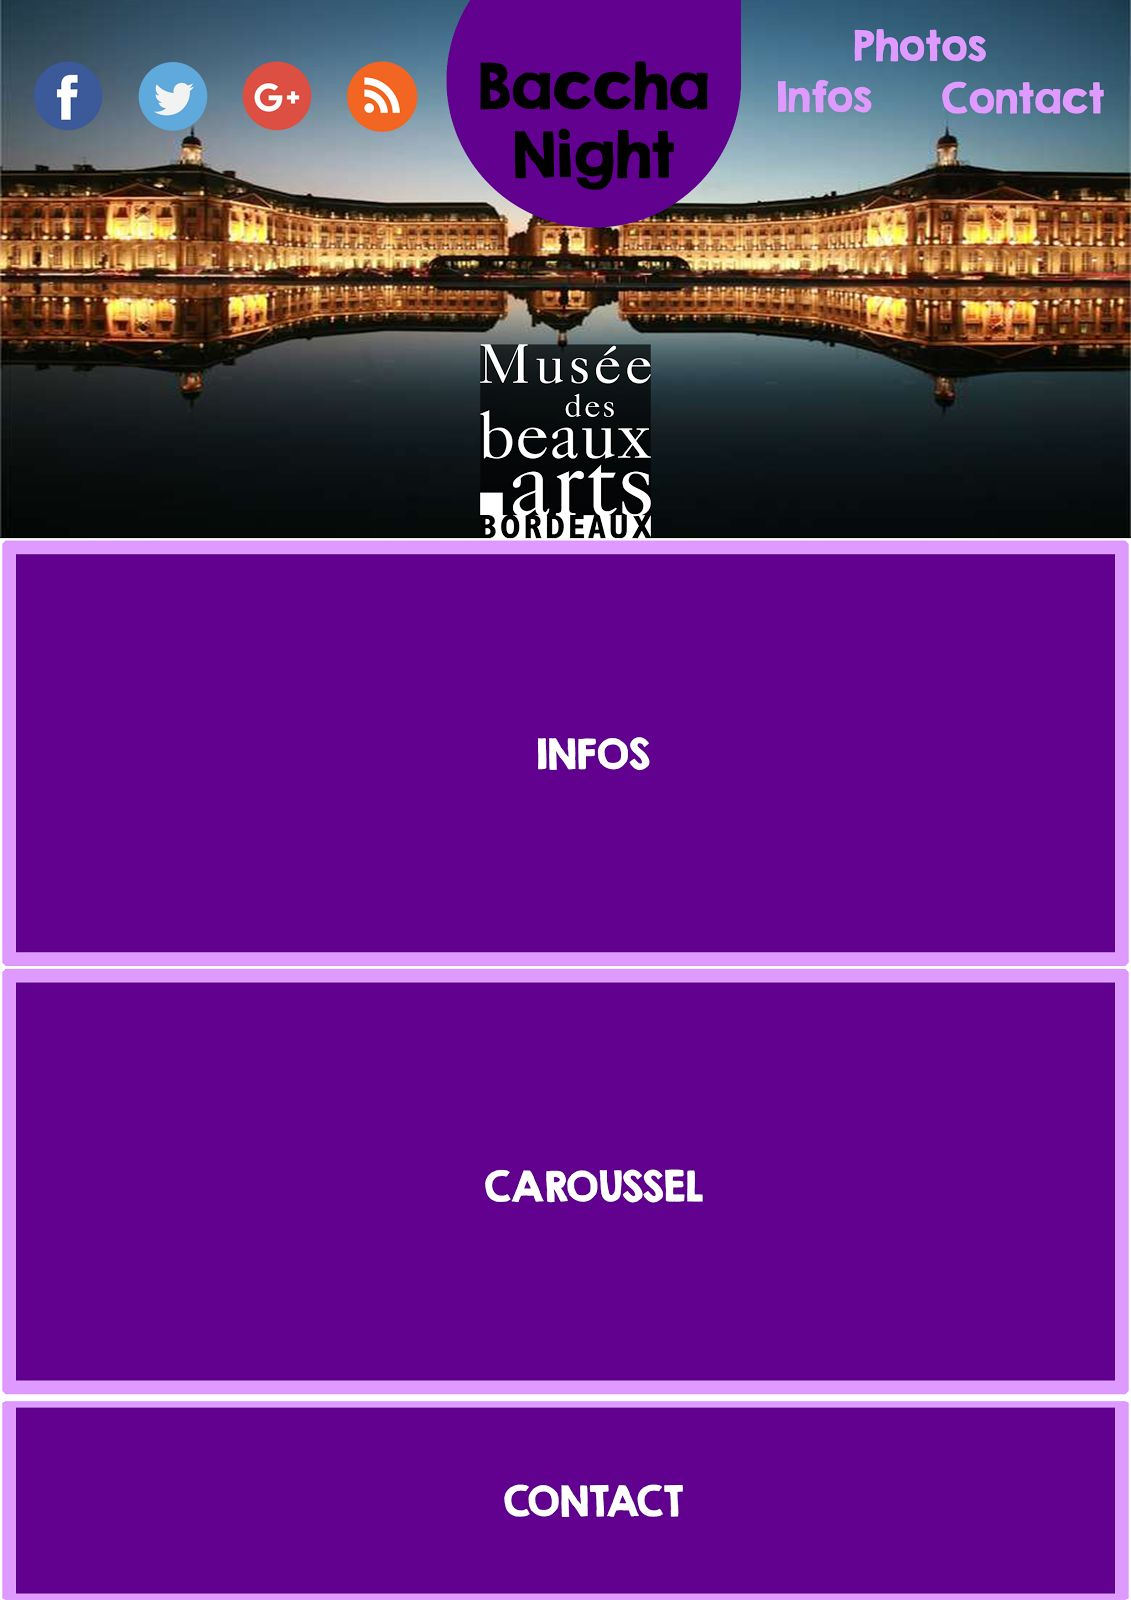
\includegraphics[width=\textwidth, height=\textheight, keepaspectratio=true]{maquette.png}}
\end{center}

%----------------------------------------------------------------------------------------
%	Annexe
%----------------------------------------------------------------------------------------

\section{Annexe}

\begin{center}
  \makebox[\textwidth]{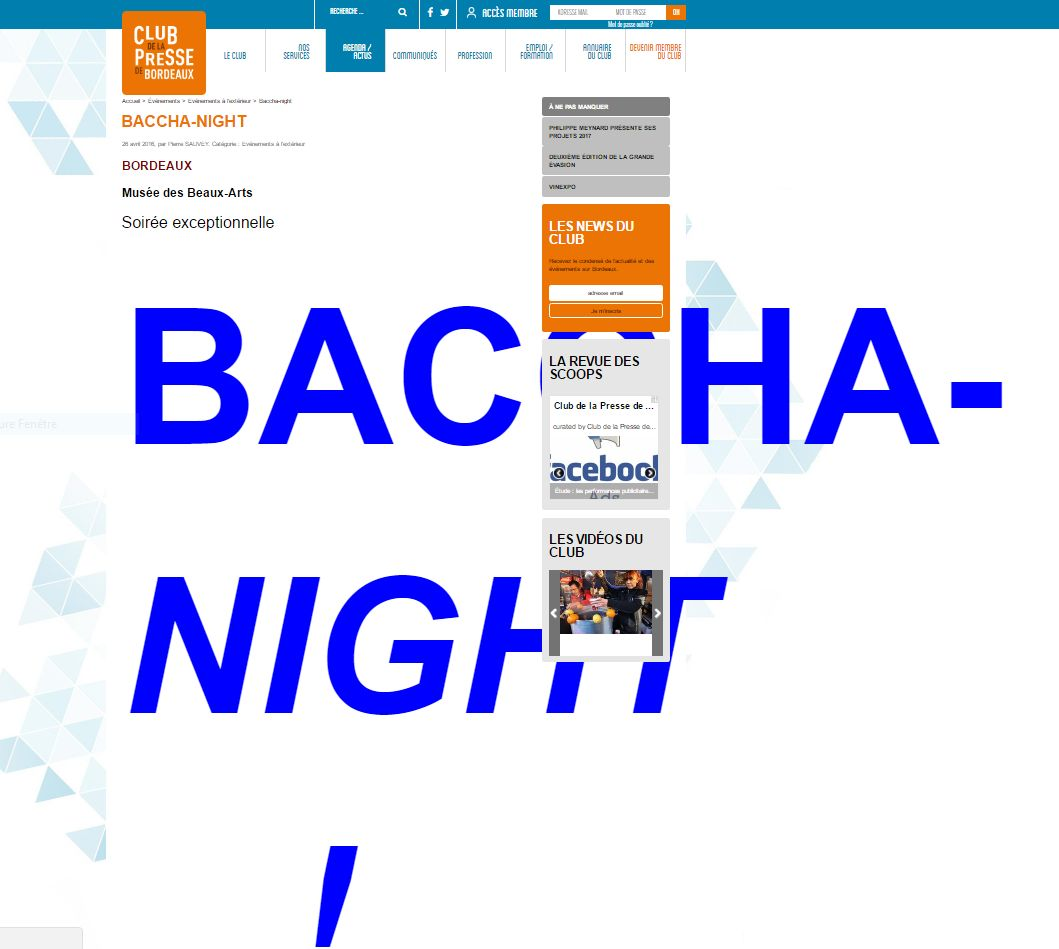
\includegraphics[width=\textwidth, height=\textheight, keepaspectratio=true]{annexe1.png}}
\end{center}

\begin{center}
  \makebox[\textwidth]{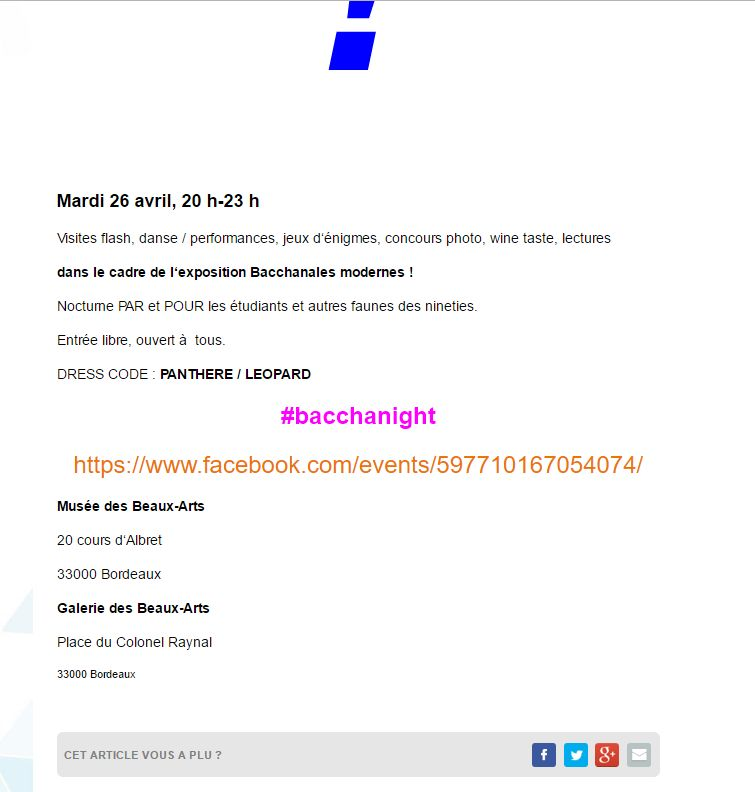
\includegraphics[width=\textwidth, height=\textheight, keepaspectratio=true]{annexe2.png}}
\end{center}

\end{document}
